\section{1174057 Alit Fajar Kurniawan}
\subsection{Teori}
	\subsubsection{Jelaskan apa itu binary classification dilengkapi ilustrasi gambar sendiri}
	\par Binary classification merupakan jenis masalah pembelajaran mesin yang paling sederhana.
	mengkalrifikasikan elemen-elemen dari himpunan yang diberikan kedalam dua kelompok berdasarkan aturan klarifikasi. Contoh yang paling sederhana dalam binary classification yaitu mendeteksi dan mendiagnosa. Berikut contoh gambar Binary Classification, gambar 2.1
		\begin{figure}[H]
			\centering
			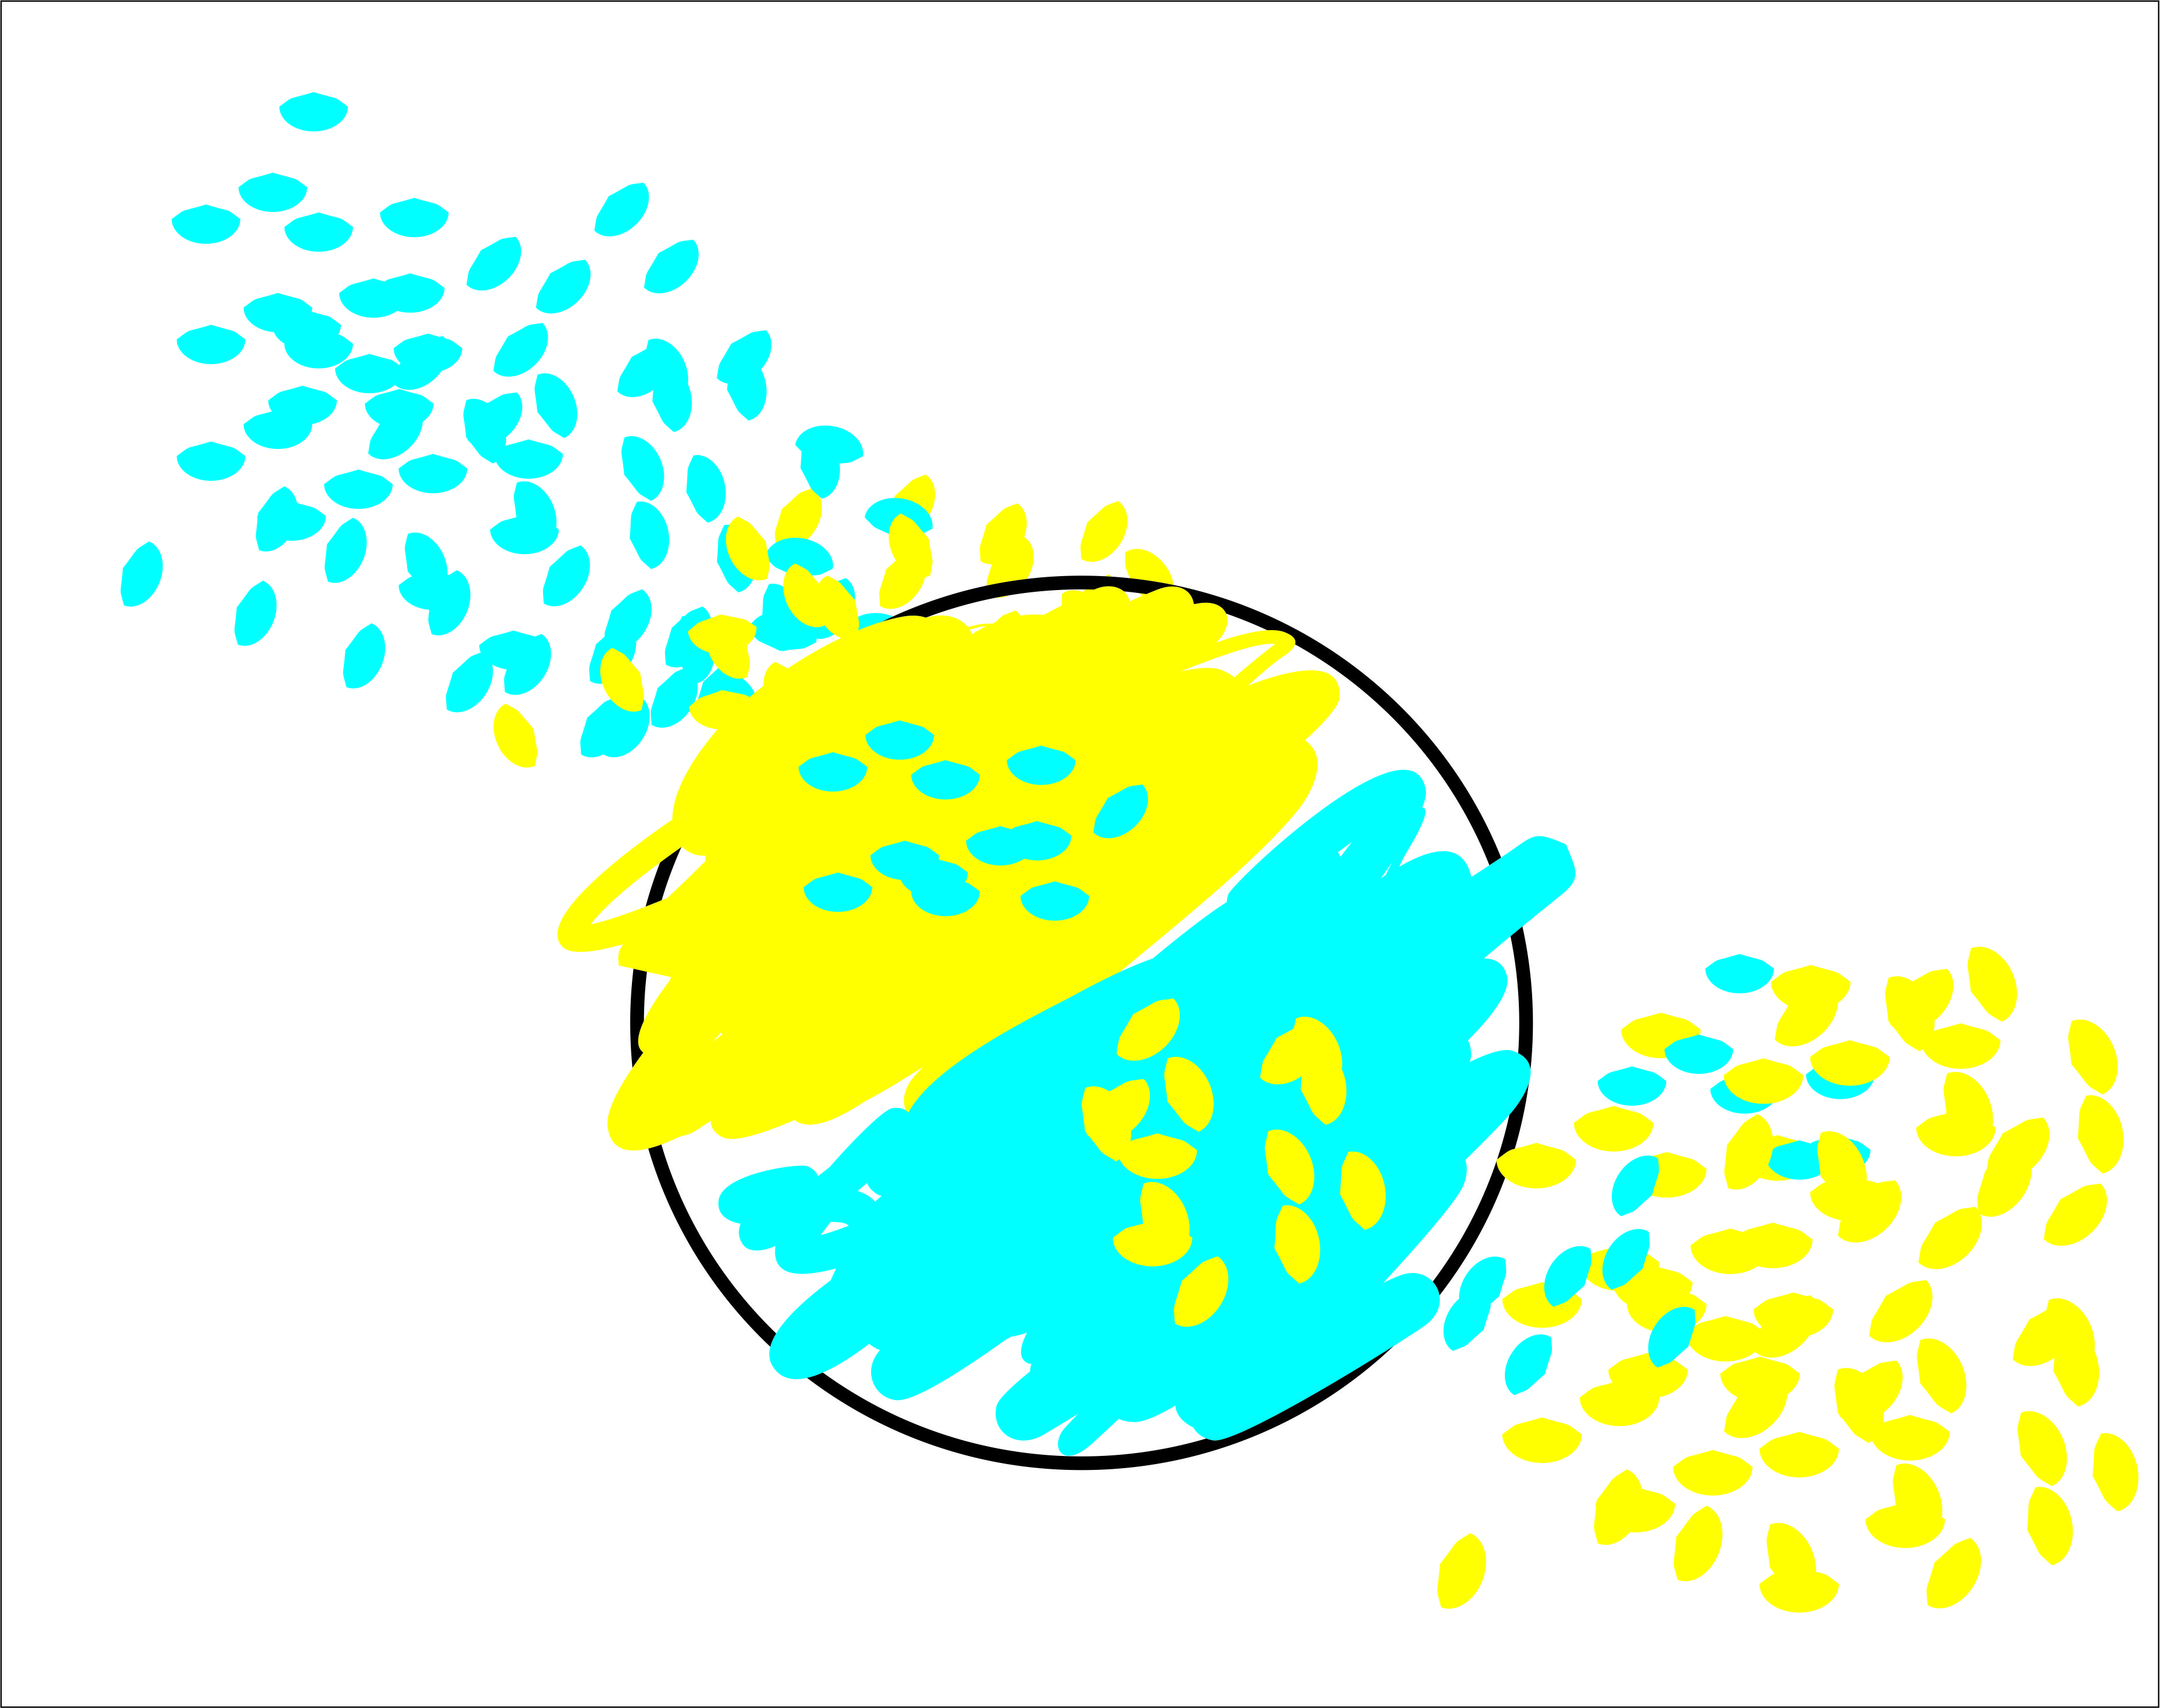
\includegraphics[width=0.5\textwidth]{figures/1174057/chapter2/1.jpg}
			\caption{Klasifikasi Binari}
			\label{print}
		\end{figure}

	\subsubsection{Jelaskan apa itu supervised learning dan unsupervised learning dan clustering dengan ilustrasi gambar sendiri}
	\par Supervised Learning merupakan paradigma belajar yang berkaitan dengan studi tentang bagaimana
	komputer dan sistem alami seperti manusia belajar \cite{zhou2018brief}. Tujuannya untuk menyimpulkan pemetaan fungsional berdasarkan serangkaian pelatihan atau mengelompokkan suatu data ke data yang sudah ada. Berikut contoh gambar Supervised Learning
		%\begin{figure}[H]
		%	\centering
		%	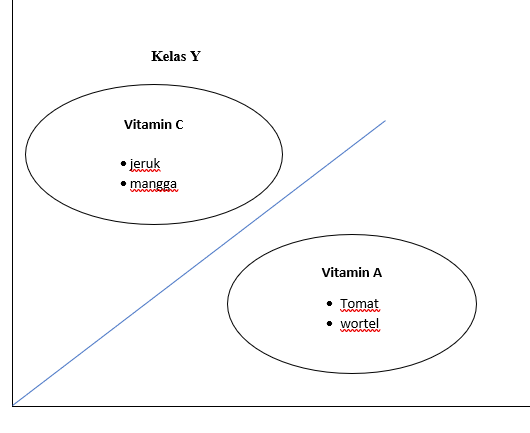
\includegraphics[width=1\textwidth]{figures/1174057/chapter2/2.png}
		%	\caption{Supervised Learning}
		%	\label{print}
		%\end{figure}
	\par Unsupervised Learning merupakan sebuah data yang belum ditentukan variabelnya jadi hanya berupa data saja. Dalam sebuah kasus Unsupervised Learning adalah aggap saja anda belum pernah membeli buku sama sekali dan pada suatu hari anda telah membeli buku dengan sangat banyak dalam kategori yang berbeda. Sehingga buku tersebut belum di kategorikan dan hanya berupa data buku saja.
		%\begin{figure}[H]
		%	\centering
		%	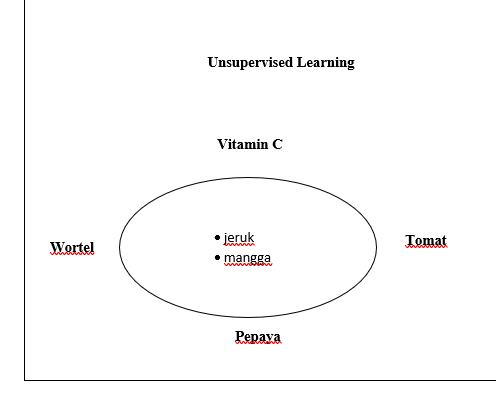
\includegraphics[width=1\textwidth]{figures/1174057/chapter2/3.png}
		%	\caption{Supervised Learning}
		%	\label{print}
		%\end{figure}
	\par Clustering merupakan metode pengelompokan data, clustering juga suatu proses partisi satu set objek data ke dalam himpunan bagian yang disebut dengan cluster. Objek yang pada cluster memiliki kesamaan secara karakteristik antara satu sama lainnya dan berbeda dengan cluster yang lain.
		%\begin{figure}[H]
		%	\centering
		%	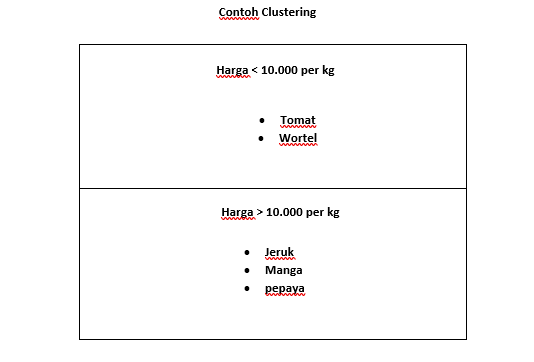
\includegraphics[width=1\textwidth]{figures/1174057/chapter2/4.png}
		%	\caption{Supervised Learning}
		%	\label{print}
		%\end{figure}

\subsection{Praktek}

\subsection{Penanganan Error}

\subsection{Bukti Tidak Plagiat}
		\begin{figure}[H]
			\centering
			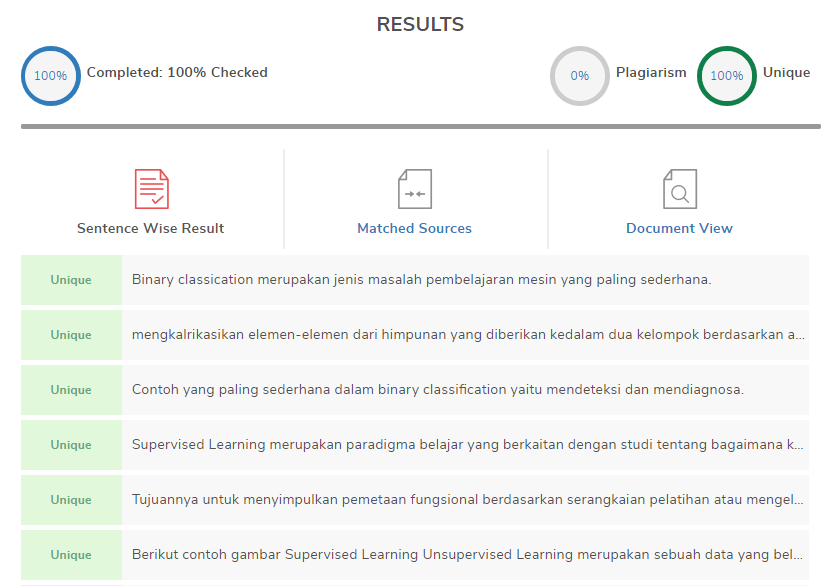
\includegraphics[width=1\textwidth]{figures/1174057/chapter2/plagiat.png}
			\caption{Plagiarisme}
			\label{print}
		\end{figure}


